\documentclass[12pt,letterpaper]{article}
\usepackage[utf8]{inputenc}
\usepackage[spanish]{babel}
\usepackage{graphicx}
\usepackage[left=2cm,right=2cm,top=2cm,bottom=2cm]{geometry}
\usepackage{graphicx} % figuras
% \usepackage{subfigure} % subfiguras
\usepackage{float} % para usar [H]
\usepackage{amsmath}
%\usepackage{txfonts}
\usepackage{stackrel} 
\usepackage{multirow}
\usepackage{enumerate} % enumerados
\renewcommand{\labelitemi}{$-$}
\renewcommand{\labelitemii}{$\cdot$}
% \author{}
% \title{Caratula}
\begin{document}

% Fancy Header and Footer
% \usepackage{fancyhdr}
% \pagestyle{fancy}
% \cfoot{}
% \rfoot{\thepage}
%

% \usepackage[hidelinks]{hyperref} % CREA HYPERVINCULOS EN INDICE

% \author{}
\title{Caratula}

\begin{titlepage}
\begin{center}
\large{UNIVERSIDAD PRIVADA DE TACNA}\\
\vspace*{-0.025in}
\begin{figure}[htb]
\begin{center}

\includegraphics[width=8cm]{./images/logo}
\end{center}
\end{figure}
\vspace*{0.15in}
INGENIERIA DE SISTEMAS \\

\vspace*{0.5in}
\begin{large}
TITULO:\\
\end{large}

\vspace*{0.1in}
\begin{Large}
\textbf{Informe de Laboratorio 03: Creando un Reporte Interactivo en PowerBI} \\
\end{Large}

\vspace*{0.3in}
\begin{Large}
\textbf{CURSO:} \\
\end{Large}

\vspace*{0.1in}
\begin{large}
INTELIGENCIA DE NEGOCIOS\\
\end{large}

\vspace*{0.3in}
\begin{Large}
\textbf{DOCENTE(ING):} \\
\end{Large}

\vspace*{0.1in}
\begin{large}
 Patrick Cuadros Quiroga\\
\end{large}

\vspace*{0.2in}
\vspace*{0.1in}
\begin{large}

\begin{flushleft}
Alumno: \\
Moreno Mulluni, Luis Angel 		\hfill	(2017057864) \\

\centering  %CENTRA UN TEXTO
\vspace*{0.9in}
\begin{large}
Tacna\\ 27-04-2019
\end{large}


\end{flushleft}
\end{large}
\end{center}

\end{titlepage}


\tableofcontents % INDICE
\thispagestyle{empty} % INDICE SIN NUMERO
\newpage
\setcounter{page}{1} % REINICIAR CONTADOR DE PAGINAS DESPUES DEL INDICE

\section{Abstract}

Business Intelligence delivers a rich set of benefits that drive significant and tangible return on investment. It removes the complexity of converting raw data into meaningful business intelligence by giving organizations the power to transform data from multiple sources into accurate, consumable information that can be shared securely throughout the enterprise. It enables users to make informed business decisions quickly and confidently by providing the query and reporting tools they need to find, share, manage, publish and analyze information. The goal of Business Intelligence is to enable management to make more intelligent decisions on the basis of knowledge extracted from data. Does this mean that having data is always good, that having more data and extracting more Knowledge from it is better, and that knowledge can be derived only from data?\newline

The paper also aims at describing processes of building Business Intelligence (BI) systems. Taking the BI systems specifics into consideration, the author presents a suggested methodology for the systems creation and implementation in organizations. The considerations are focused on the objectives and functional areas of the BI in organizations. Hence, in this context the approach to be used while building and implementing the BI involves two major stages that are of interactive nature, i.e. BI creation and BI “consumption”. A large part of the article is devoted to presenting Objectives and tasks that are realized while building and implementing BI.\newline

\textbf{Key words:} Business Intelligence, business decision-making, analytics, memory, monitoring.
\section{Introducción} 
\vspace{12mm} %5mm vertical space
Actualmente las organizaciones sin importar cuál sea su giro, se encuentran en una incertidumbre
permanente, debido al impacto de la globalización en los mercadosi
, estos cambios constantes en el
mercado y en los competidores, impactan a la empresa que ha obtenido “buenos resultados” durante años,
por lo que se ve en la necesidad de tener que cambiar de manera radical sus procesos, productos y/ o
servicios, en general la manera de llevar la administración de las organizaciones, pues estos cambios
(tecnológicos, sociales, culturales, económicos, etc.) obligan a generar indicadores, que den un mayor grado
de certeza en la toma de decisiones y así reducir el riesgo de fallar, de perder inversión o de no ser
competitivo, pues son estos algunas de las principales áreas que deberán estar vigilándose periódicamenteii
.
Tradicionalmente la evaluación de un negocio se basa en su liquidez económica, esto solo considera los
aspectos financieros, sin considerar el entorno organizacional, es decir, comúnmente no se toma en cuenta si
los clientes se encuentran satisfechos con los productos o servicios que las empresas generan, más aun no se
toma en cuenta si los procesos internos son los más adecuados o si la empresa está aprendiendo y
desarrollándose en base a ese aprendizaje.\newline


En la práctica es común que no se puedan identificar con claridad los puntos fuertes y débiles de la empresa
para la que se labora, ya que no es fácil analizar una situación cuando se está inmerso en ella, de hecho
seguramente para los directivos y propietarios de una organización será muy difícil encontrarse frente al
dilema “cambiar o morir”, mayormente si durante mucho tiempo se ha venido actuando de una manera
rutinaria, pero al confrontar situaciones relacionadas con: sacrificar margen de ganancia, perdida de ventaja
competitiva, crisis en el modelo estructural del negocio, por citar solo algunos puntos críticos para las
empresas, por esto se vuelve apremiante la necesidad de encontrar la manera de evaluar el desempeño de las
empresas.\newline
Este desempeño no puede medirse de la misma manera en todas las empresas aunque pertenezcan al
mismo sector como lo menciona Rouquette (2014) en su investigación de Análisis de varianza.
Por lo anterior es preciso tener claro qué es y para qué sirve la estrategia, de este modo “La estrategia
consiste en hacer un profundo análisis tanto de la organización como del entorno para definir un plan de
acción que lleve a mejorar la posición sobre los competidores”iv por otra parte la existencia de diferentes
herramientas que puedan complementar y mejorar estudios encaminados a validar la factibilidad de
emprendimiento. \newline


\vspace{16mm} %5mm vertical space
\section{Marco Teórico} 
\subsection{Business Intelligence}

Business Intelligence es la habilidad para transformar los datos en información, y la información en conocimiento, de forma que se pueda optimizar el proceso de toma de decisiones en los negocios.\newline

\begin{center}
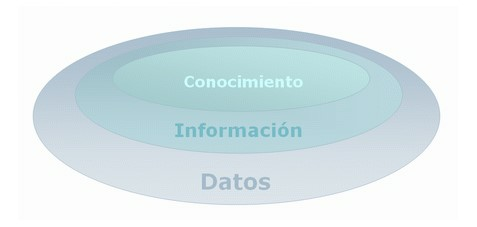
\includegraphics{images/bi/bi-cid}\\
\end{center}

Desde un punto de vista más pragmático, y asociándolo directamente con las tecnologías de la información, podemos definir Business Intelligence como el conjunto de metodologías, aplicaciones y tecnologías que permiten reunir, depurar y transformar datos de los sistemas transaccionales e información desestructurada (interna y externa a la compañía) en información estructurada, para su explotación directa (reporting, análisis OLTP / OLAP, alertas) o para su análisis y conversión en conocimiento, dando así soporte a la toma de decisiones sobre el negocio.\newline

La inteligencia de negocio actúa como un factor estratégico para una empresa u organización, generando una potencial ventaja competitiva, que no es otra que proporcionar información privilegiada para responder a los problemas de negocio: entrada a nuevos mercados, promociones u ofertas de productos, eliminación de islas de información, control financiero, optimización de costes, planificación de la producción, análisis de perfiles de clientes, rentabilidad de un producto concreto, etc.\newline

Los principales productos de Business Intelligence que existen hoy en día son:

\begin{itemize}
\item Cuadros de Mando Integrales (CMI).
\item Sistemas de Soporte a la Decisión (DSS).
\item Sistemas de Información Ejecutiva (EIS).
\end{itemize}

Por otro lado, los principales componentes de orígenes de datos en el Business Intelligence que existen en la actualidad son:

\begin{itemize}
\item Datamart.
\item Datawarehouse.
\end{itemize}

Los sistemas y componentes del BI se diferencian de los sistemas operacionales en que están optimizados para preguntar y divulgar sobre datos. Esto significa típicamente que, en un datawarehouse, los datos están desnormalizados para apoyar consultas de alto rendimiento, mientras que en los sistemas operacionales suelen encontrarse normalizados para apoyar operaciones continuas de inserción, modificación y borrado de datos. En este sentido, los procesos ETL (extracción, transformación y carga), que nutren los sistemas BI, tienen que traducir de uno o varios sistemas operacionales normalizados e independientes a un único sistema desnormalizado, cuyos datos estén completamente integrados.\newline

En definitiva, una solución BI completa permite:

\begin{itemize}
\item \textbf{Observar} ¿qué está ocurriendo?
\item \textbf{Comprender} ¿por qué ocurre?
\item \textbf{Predecir} ¿qué ocurriría?
\item \textbf{Colaborar} ¿qué debería hacer el equipo?
\item \textbf{Decidir} ¿qué camino se debe seguir?\newline
\end{itemize}

\begin{center}
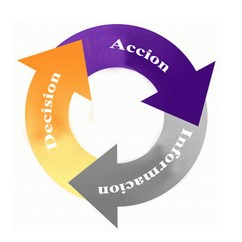
\includegraphics{images/bi/bi-dai}\newline
\end{center}

\subsection{Business Analytics}

Business Analytics es “el estudio de datos a través de análisis estadísticos y de operaciones, la formación de modelos predictivos, la aplicación de técnicas de optimización y la comunicación de estos resultados a clientes, socios comerciales y ejecutivos de universidades”. Business Analytics requiere métodos cuantitativos y pruebas.\newline

% Datos basados ​​en modelos de negocios y toma de decisiones; como tal, Business Analytics requiere el uso de Big Data.\newline

\begin{center}

\includegraphics{images/ba/ba-c}\newline
\end{center}

\textbf{Beneficios de la toma de decisiones basada en datos con Business Analytics}\newline

Las empresas utilizan Business Analytics (BA) para tomar decisiones basadas en datos. La información obtenida por BA permite a estas empresas automatizar y optimizar sus procesos de negocios. De hecho, las empresas basadas en datos que utilizan Business Analytics logran una ventaja competitiva porque son capaces de utilizar los conocimientos para:

\begin{itemize}
\item Realizar minería de datos (explorar datos para encontrar nuevos patrones y relaciones).
\item Análisis estadístico completo y análisis cuantitativo para explicar por qué ocurren ciertos resultados.
\item Probar decisiones anteriores utilizando pruebas A / B y pruebas multivariadas.
\item Utilice el modelado predictivo y el análisis predictivo para pronosticar resultados futuros.
\end{itemize}

Business Analytics también brinda soporte a las compañías en el proceso de tomar decisiones tácticas proactivas, y BA hace posible que esas compañías automaticen la toma de decisiones para respaldar las respuestas en tiempo real.\newline

Una forma de clasificar la Analítica Empresarial podrían ser estas tres áreas más o menos superpuestas:

\begin{itemize}
\item \textbf{Analítica Descriptiva o Descriptive Analytics.}\\ Utiliza los datos para explicar el pasado. Consiste en preparar y analizar datos históricos para identificar patrones y tendencias. Técnicas como modelos de regresión, el modelado de datos y visualización suelen ser usados en la Analítica Descriptiva.
\item \textbf{Analítica Predictiva o Predictive Analytics.}\\ Utiliza los datos para determinar que puede pasar en el futuro. La Analítica Predictiva permite determinar la probabilidad asociada a eventos futuros a partir del análisis de la información disponible (presente y pasada), además permite descubrir relaciones entre los datos que normalmente no es detectada con un análisis menos sofisticado. Técnicas como la minería de datos (data mining) y los modelos predictivos son utilizados.
\item \textbf{Analítica Prescriptiva o Prescriptive Analytics.}\\ Utiliza los datos para prescribir aquellas acciones que incrementen nuestras posibilidades de obtener los mejores resultados. La Analítica Prescriptiva determina nuevos forma de operar que permitan alcanzar nuestros objetivos de negocio. Técnicas como la optimización o la simulación son utilizadas, aunque normalmente se requiere la creación de un modelo predictivo previo.
\end{itemize}

Por tanto, la analítica empresarial nos permite:

\begin{itemize}
\item Alcanzar objetivos empresariales a partir del análisis de grandes volúmenes de datos.
\item Detectar tendencias y realizar pronósticos a partir de modelos predictivos.
\item Utilizar estos modelos predictivos para optimizar los procesos de negocio.
\end{itemize}


\textbf{Desafíos con Business Analytics}\newline

John Jordan, de la Universidad de Penn State, describió los desafíos con Business Analytics: existe “un mayor potencial para la invasión de la privacidad, una mayor exposición financiera en los mercados que se mueven rápidamente, un mayor potencial para confundir el ruido con una visión real, y un mayor riesgo de gastar mucho dinero y tiempo persiguiendo problemas u oportunidades mal definidas ”. Otros desafíos con el desarrollo e implementación de Business Analytics incluyen:\newline

\begin{itemize}
\item Propiedad de ejecutivos: Business Analytics requiere la aceptación del liderazgo sénior y una estrategia corporativa clara para integrar modelos predictivos.
\item Participación de TI: la infraestructura tecnológica y las herramientas deben ser capaces de manejar los datos y los procesos de Business Analytics.
\item Datos de producción disponibles frente a datos de modelado limpios: observe la infraestructura tecnológica que restringe los datos disponibles para el modelado histórico, y conozca la diferencia entre los datos históricos para el desarrollo de modelos y los datos en tiempo real en producción.
\item Oficina de gestión de proyectos (PMO): la estructura de gestión de proyectos correcta debe estar implementada para implementar modelos predictivos y adoptar un enfoque ágil.
\item Participación y compra del usuario final: los usuarios finales deben participar en la adopción de Business Analytics y tener un interés en el modelo predictivo.
\item Gestión de cambios: las organizaciones deben estar preparadas para los cambios que Business Analytics aporta a las operaciones comerciales y tecnológicas actuales.
\item Explicabilidad frente a la "elevación perfecta": equilibre la construcción de modelos estadísticos precisos con la posibilidad de explicar el modelo y cómo producirá resultados.\newline
\end{itemize}

\textbf{Mejores Prácticas de Business Analytics}\newline

Adoptar e implementar Business Analytics no es algo que una empresa pueda hacer de la noche a la mañana. Pero, si una empresa sigue algunas de las mejores prácticas para Business Analytics, obtendrán los niveles de conocimiento que buscan y serán más competitivas y exitosas. Aquí enumeramos algunas de las mejores prácticas más importantes para Business Analytics, aunque su organización tendrá que determinar cuáles son las mejores prácticas que se adaptan a sus necesidades.

\begin{itemize}
\item Conozca el objetivo de utilizar Business Analytics. Defina su caso de uso comercial y el objetivo antes de tiempo.
\item Define tus criterios para el éxito y el fracaso.
\item Seleccione su metodología y asegúrese de conocer los datos y los factores internos y externos relevantes.
\item Valide modelos utilizando sus criterios predefinidos de éxito y fracaso.
\end{itemize}

Business Analytics es fundamental para seguir siendo competitivo y lograr el éxito. Cuando implementa las mejores prácticas de BA y obtiene la aceptación de todas las partes interesadas, su organización se beneficiará de la toma de decisiones basada en datos.\newline

\begin{center}
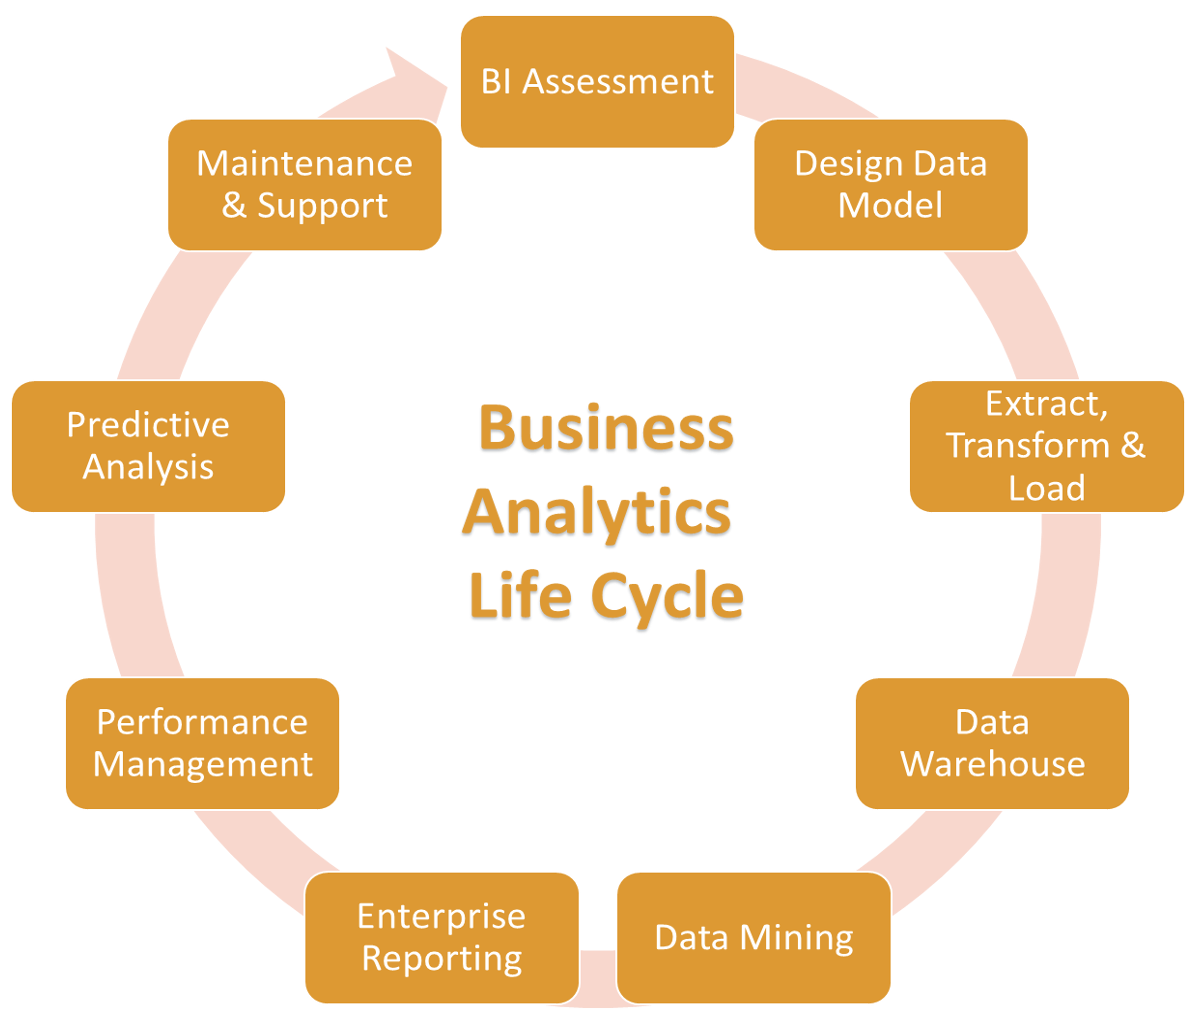
\includegraphics[width=0.6\columnwidth]{images/ba/ba-lc}
\end{center}

\end{document}
